\begin{problem}{Equilibrium Point /\textbackslash/\textbackslash}{standard input}{standard output}{3 seconds}{512 megabytes}

Consider a balanced bracket sequence $s$ with one type of brackets: `\t{(}' and `\t{)}'.

There is a common geometrical representation of such a sequence. Starting at the point $(0, 0)$, you draw a polyline, for each bracket moving along a vector $(1, 1)$ if it is an opening bracket, and along $(1, -1)$ if it is a closing bracket.


\begin{center}
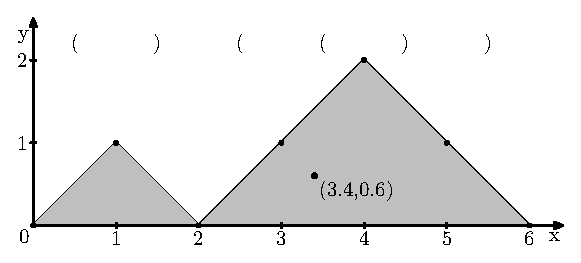
\includegraphics{equilibrium.0.eps}
\end{center}


Consider an area between this curve and the line $y=0$. It is a set of polygons. This area has its center of mass at some point $(x, y)$. Note that the center of mass might be outside of the area.

You are to solve the reverse problem. Given the length $n$ and a point $(x, y)$, find any balanced bracket sequence of length $n$ such that the center of mass of its geometrical representation is located at $(x, y)$.

\InputFile
The first line contains three numbers $n$, $x$, and $y$~($n$ is an even integer, $2 \le n \le 36$; $0 < x, y < n$)~--- the length of the desired sequence and the coordinates of the desired center of mass.

It is guaranteed that $(x, y)$ is the center of mass of some balanced bracket sequence of length $n$, with Euclidean-distance error of no more than $10^{-9}$.

\OutputFile
Output a balanced bracket sequence with brackets `\t{(}' and `\t{)}' of length $n$ such that the center of mass of its geometrical representation is located at the point $(x, y)$, with Euclidean-distance error of no more than $10^{-7}$.

\Example

\begin{example}
\exmpfile{example.01}{example.01.a}%
\end{example}

\end{problem}

